\section{Bayesian Networks}
All probabilistic inference and learning methods are based on the repeated application of basic rules of probability theory.
However, as the number of random variables increases, the complexity of representing and manipulating probability distributions grows exponentially.
Probabilistic graphical models provide a convenient framework to represent and manipulate complex probability distributions.
\\\\Bayesian Networks (BNs) are a formalism to represent probabilistic relationships among a set of random variables.
They allow to:
\begin{itemize}
    \item Visualize the structure of a probabilistic model;
    \item Discover properties of the model (e.g., conditional independencies);
    \item Efficiently perform probabilistic inference and learning, using the structure of the graph;
    \item Represent multiple distrubutions with the same graph, independently of their qualitative aspects
    (e.g., discrete vs continuous variables).
\end{itemize}

\subsection{Bayesian Networks structure}
A Bayesian Network (BN) structure $\mathcal{G}$ is a directed acyclic graph (DAG) where:
\begin{itemize}
    \item Each node represents a random variable;
    \item Each directed edge represent a direct dependency between the two connected variables;
\end{itemize}
It's important to note that the absence of an edge between two nodes doesn't imply independence.
\\\\The given structure $\mathcal{G}$ of a BN encodes these independence assumptions:
\[ \mathcal{I}_l(\mathcal{G}) = \{ \forall i\; \boldsymbol{x}_i \perp \text{NonDescendants}_{\boldsymbol{x}_i} | \text{Parents}_{\boldsymbol{x}_i} \} \]
Each variable $\boldsymbol{x}_i$ is independent of its non-descendants given its parents. 

\begin{figure}[H]
\centering
    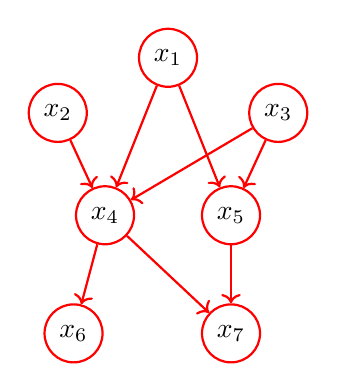
\begin{tikzpicture}[
        node/.style={circle, draw=red, thick, minimum size=18pt},
        arrow/.style={->, red, thick}
    ]
    % Nodes
    \node[node] (x1) at (0, 3.5) {$x_1$};
    \node[node] (x2) at (-1.4, 2.8) {$x_2$};
    \node[node] (x3) at (1.4, 2.8) {$x_3$};
    \node[node] (x4) at (-0.8, 1.5) {$x_4$};
    \node[node] (x5) at (0.8, 1.5) {$x_5$};
    \node[node] (x6) at (-1.2, 0) {$x_6$};
    \node[node] (x7) at (0.8, 0) {$x_7$};
    % Edges
    \draw[arrow] (x1) -- (x4);
    \draw[arrow] (x1) -- (x5);
    \draw[arrow] (x2) -- (x4);
    \draw[arrow] (x3) -- (x4);
    \draw[arrow] (x3) -- (x5);
    \draw[arrow] (x4) -- (x6);
    \draw[arrow] (x4) -- (x7);
    \draw[arrow] (x5) -- (x7);
    \end{tikzpicture}
    \caption{Example of Bayesian Network}
\end{figure}
\subsubsection{Independency Map}
\defib{Independency Map}{
    \begin{itemize}
        \item Let $p$ be a distribution over a set of random variables $\boldsymbol{X}$;
        \item Let $\mathcal{I}(p)$ be the set of independencies that hold in $p$;
    \end{itemize}
    We say that $\mathcal{G}$ is an \textbf{Independency Map} (I-map) for $p$ if $p$ satisfies
    the local independencies encoded in $\mathcal{G}$:
    \[ \mathcal{I}_l(\mathcal{G}) \subseteq \mathcal{I}(p) \]
}
This means that all independencies encoded in the graph $\mathcal{G}$ hold in the distribution $p$.
There can be additional independencies in $p$ that are not encoded in $\mathcal{G}$.

\subsubsection{Factorization}
We say that a distribution $p$ \textbf{factorizes} according to a BN structure $\mathcal{G}$ if $p$ can be expressed as:
\[ p(\boldsymbol{x}_1, \boldsymbol{x}_2, \ldots, \boldsymbol{x}_m) = \prod_{i=1}^{m} p(\boldsymbol{x}_i | \text{Parents}_{\boldsymbol{x}_i}) \]
We have that $\mathcal{G}$ is an I-map for $p$ if and only if $p$ factorizes according to $\mathcal{G}$.
\begin{comment}
%#TODO: Add proof here
\begin{proof}
\end{proof}
\end{comment}

\subsection{Bayesian Network definition}
A Bayesian Network (BN) is a pair $\mathcal{B} = (\mathcal{G}, \mathcal{P})$, where:
\begin{itemize}
    \item $\mathcal{G}$ is a directed acyclic graph (DAG) representing the structure of the BN;
    \item $\mathcal{P}$ is a set of conditional probability distributions (CPDs) associated with the nodes in the graph.
\end{itemize}
$P$ must factorize according to $\mathcal{G}$:
\[ P(\boldsymbol{x}_1, \boldsymbol{x}_2, \ldots, \boldsymbol{x}_m) = \prod_{i=1}^{m} P(\boldsymbol{x}_i | \text{Parents}_{\boldsymbol{x}_i}) \]

\paragraph{Example:}
Consider the following BN structure:
\begin{figure}[H]
\centering
    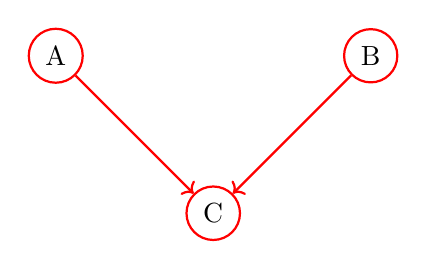
\begin{tikzpicture}[
        node/.style={circle, draw=red, thick, minimum size=18pt},
        arrow/.style={->, red, thick}
    ]
    % Nodes
    \node[node] (A) at (-2, 1) {A};
    \node[node] (B) at (2, 1) {B};
    \node[node] (C) at (0, -1) {C};
    % Edges
    \draw[arrow] (A) -- (C);
    \draw[arrow] (B) -- (C);
    \end{tikzpicture}
    \caption{Example of Bayesian Network structure}
\end{figure}
\begin{itemize}
    \item Gene $A$ and Gene $B$ are independent;
    \item Gene $C$ can be influenced by both Gene $A$ and Gene $B$;
\end{itemize}
\begin{center}
    \begin{minipage}{0.4\textwidth}
        \centering
        \label{tab:cpdGeneA}
        \begin{tabular}{c|c|c}
            Gene &  Value & P(value)\\ 
            \hline
            A & active   & 0.3\\
            A & inactive & 0.7\\
        \end{tabular}
        \captionof{table}{CPD for Gene A}
    \end{minipage}
    \hfill
    \begin{minipage}{0.4\textwidth}
    \centering
        \label{tab:cpdGeneB}
        \begin{tabular}{c|c|c}
            Gene &  Value & P(value)\\ 
            \hline
            B & active   & 0.3\\
            B & inactive & 0.7\\
        \end{tabular}
        \captionof{table}{CPD for Gene B}
    \end{minipage}
\end{center}

\begin{center}
\begin{tabular}{|c|c|cc|cc|}
\hline
 & & \multicolumn{4}{c|}{A} \\
 & & \multicolumn{2}{c|}{active} & \multicolumn{2}{c|}{inactive} \\
\cline{3-6}
 & & \multicolumn{2}{c|}{B} & \multicolumn{2}{c|}{B} \\
 & & active & inactive & active & inactive \\
\hline
\multirow{2}{*}{C}
 & active   & 0.9 & 0.6 & 0.7 & 0.1 \\
 & inactive & 0.1 & 0.4 & 0.3 & 0.9 \\
\hline
\end{tabular}
\captionof{table}{Conditional Probability Table for Gene C}
\end{center}

\subsection{D-separation}
Before introducing the concept of D-separation, we need to better understand the concept of independence and conditional independence.
We will then present the basic structures that can appear in a BN.

\subsubsection{Independence and conditional independence}
\defib{Independence}{
We usually say that, two variables $a, b$ are independent (written $a \perp b|\empty$) if:
    \[ P(a, b) = P(a) P(b) \]
}
\defib{Conditional independence}{
    We say that two variables $a, b$ are conditionally independent given a third variable $c$ (written $a \perp b | c$) if:
    \[ P(a, b | c) = P(a | c) P(b | c) \]
}
Both independence and conditional independence can be verified by applying basic rules of probability.
Instead, BN allow to verify this properties through the concept of D-separation.

\subsubsection{Tail-to-tail connection}
In a tail-to-tail connection, two variables $a$ and $b$ are connected through a common parent variable $c$.
It is called tail-to-tail because the node $c$ has two outgoing edges (tails) pointing to $a$ and $b$.
\begin{figure}[H]
\centering
    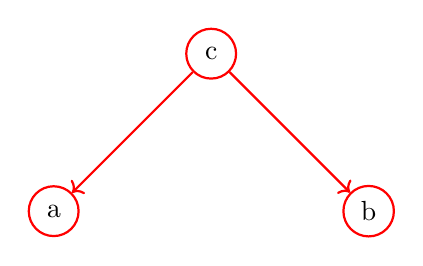
\begin{tikzpicture}[
        node/.style={circle, draw=red, thick, minimum size=18pt},
        arrow/.style={->, red, thick}
    ]
    % Nodes
    \node[node] (C) at (0, 1) {c};
    \node[node] (A) at (-2, -1) {a};
    \node[node] (B) at (2, -1) {b};
    % Edges
    \draw[arrow] (C) -- (A);
    \draw[arrow] (C) -- (B);
    \end{tikzpicture}
    \caption{Tail-to-tail connection}
\end{figure}
The joint distribution can be expressed as:
\begin{equation}
    \label{eq:tailToTail}
    P(a, b, c) = P(a | c) P(b| c) P(c)
\end{equation}
Given this, we want to understand the independency relationships between $a$ and $b$:
\begin{itemize}
    \item \textbf{Independent}: we need to check that $P(a, b) = P(a) P(b)$;
    To do this, we marginalize over $c$, applying the sum rule:
    \[ P(a, b) = \sum_{c} P(a, b, c) \]
    We can then substitute the joint distribution from eq \ref{eq:tailToTail}:
    \[ P(a, b) = \sum_{c} P(a | c) P(b| c) P(c) \neq P(a) P(b)\]
    So $a$ and $b$ are \textbf{not independent}.
    \item \textbf{Conditionally independent}: we need to check that $P(a, b | c) = P(a | c) P(b | c)$;
    We can apply the product rule:
    \[ P(a, b | c) = \frac{P(a, b, c)}{P(c)} \]
    We can then substitute the joint distribution from eq \ref{eq:tailToTail}:
    \[ P(a, b | c) = \frac{P(a | c) P(b| c) P(c)}{P(c)} = P(a | c) P(b | c) \]
    So $a$ and $b$ are \textbf{conditionally independent} given $c$.
\end{itemize}
We derive that, if $c$ is observed, $a$ and $b$ become independent.
\paragraph{Example:}
A classic example of tail-to-tail connection is the relationship between covid infection $c$, 
and two symptoms: fever $a$ and cough $b$.
If we observe the covid infection status, knowing whether a patient has a fever provides no 
additional information about whether they have a cough, and vice versa.
\\Variable $c$ is a common cause of both symptoms $a$ and $b$.

\subsubsection{Head-to-tail connection}
In a head-to-tail connection, variables $a$ is a parent of variable $c$, which is a parent of variable $b$.
It is called head-to-tail because $c$ has one incoming edge (head) from $a$ and one outgoing edge (tail) to $b$.
\begin{figure}[H]
\centering
    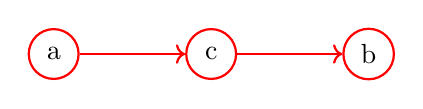
\begin{tikzpicture}[
        node/.style={circle, draw=red, thick, minimum size=18pt},
        arrow/.style={->, red, thick}
    ]
    % Nodes
    \node[node] (A) at (-2, 0) {a};
    \node[node] (C) at (0, 0) {c};
    \node[node] (B) at (2, 0) {b};
    % Edges
    \draw[arrow] (A) -- (C);
    \draw[arrow] (C) -- (B);
    \end{tikzpicture}
    \caption{Head-to-tail connection}
\end{figure}
The joint distribution can be expressed as:
\[ p(a,b,c) = p(b|c) p(c|a) p(a) \]
Note that, using Bayes' theorem, we can rewrite $p(c|a) p(a)$ as $p(a|c) p(c)$, obtaining:
\[ p(a,b,c) = p(b|c) p(a|c) p(c) \]
Given this, we want to understand the independency relationships between $a$ and $b$:
\begin{itemize}
    \item \textbf{Independent}: we need to check that $P(a, b) = P(a) P(b)$;
    We repeat the same steps as before:
    \[ P(a, b) = \sum_{c} P(a, b, c) = \sum_{c} p(b|c) p(c|a) p(a) \neq P(a) P(b)\]
    So $a$ and $b$ are \textbf{not independent}.
    \item \textbf{Conditionally independent}: we need to check that $P(a, b | c) = P(a | c) P(b | c)$;
    We repeat the same steps as before:
    \[ P(a, b | c) = \frac{P(a, b, c)}{P(c)} = \frac{p(b|c) p(c|a) p(a)}{P(c)} = P(a | c) P(b | c) \]
    So $a$ and $b$ are \textbf{conditionally independent} given $c$.
\end{itemize}
Intuitively, if we already know the value of $c$, knowing $a$ provides no additional information about $b$, and vice versa.
Differently from the tail-to-tail case, here $c$ is an intermediary variable between $a$ and $b$.
\paragraph{Example:}
A classic example of head-to-tail connection is the relationship between cloud coverage $a$, rain $c$, and getting wet $b$.
If we observe whether it is raining, knowing whether there is cloud coverage provides no additional 
information about wether we get wet. For both cloudy and clear skies, if it is raining we will get wet.

\subsubsection{Head-to-head connection}
In a head-to-head connection, variables $a$ and $b$ are both parents of variable $c$.
It is called head-to-head because $c$ has two incoming edges (heads) from $a$ and $b$.
\begin{figure}[H]
\centering
    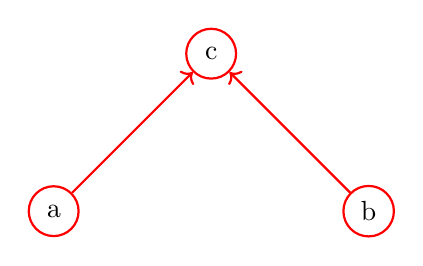
\begin{tikzpicture}[
        node/.style={circle, draw=red, thick, minimum size=18pt},
        arrow/.style={->, red, thick}
    ]
    % Nodes
    \node[node] (A) at (-2, 0) {a};
    \node[node] (B) at (2, 0) {b};
    \node[node] (C) at (0, 2) {c};
    % Edges
    \draw[arrow] (A) -- (C);
    \draw[arrow] (B) -- (C);
    \end{tikzpicture}
    \caption{Head-to-head connection}
\end{figure}
The joint distribution can be expressed as:
\[ p(a,b,c) = p(c|a,b) p(a) p(b) \]
As before, we want to understand the independency relationships between $a$ and $b$:
\begin{itemize}
    \item \textbf{Independent}:
    \[ P(a, b) = \sum_{c} P(a, b, c) = \sum_{c} p(c|a,b) p(a) p(b)\]
    Remember that summing over all possible values of $c$ gives 1, so:
    \[ P(a, b) = p(a) p(b) \]
    So $a$ and $b$ are \textbf{independent}.
    \item \textbf{Conditionally independent}:
    \[ P(a, b | c) = \frac{P(a, b, c)}{P(c)} = \frac{p(c|a,b) p(a) p(b)}{P(c)} \neq P(a | c) P(b | c) \]
    So $a$ and $b$ are \textbf{not conditionally independent} given $c$.
\end{itemize}
Intuitively, $a$ and $b$ are independent. Observing $c$ creates a dependency between $a$ and $b$.
This phenomenon is known as "explaining away": if we know that $c$ has occurred (both $a$ and $b$ could have caused it), 
observing one of the causes makes the other cause less likely.
\paragraph{Example:}
A classic example of head-to-head connection is the relationship between burglary $a$, earthquake $b$, and alarm ringing $c$.
Burglary and earthquake are independent events and are both causes of the alarm ringing.
However, if we know that the alarm has rung, observing a burglary makes an earthquake less likely.

\subsubsection{D-separation rules summary}
\begin{figure}[H]
    \usetikzlibrary{shapes.geometric,arrows.meta,positioning,backgrounds}
    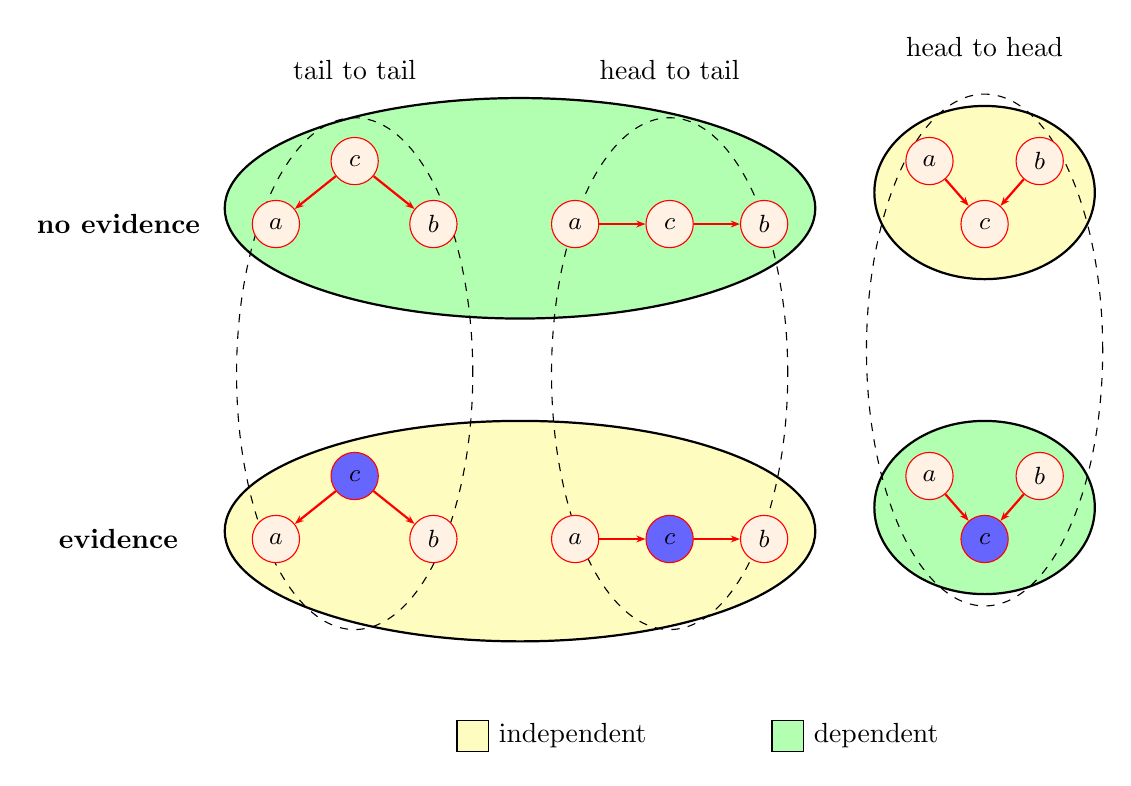
\begin{tikzpicture}[
        node distance=1cm,
        % Node Styles
        node_empty/.style={circle, draw=red, fill=orange!10, minimum size=6mm, inner sep=0pt},
        node_filled/.style={circle, draw=red, fill=blue!60, minimum size=6mm, inner sep=0pt},
        % Background Shapes
        indep_bg/.style={ellipse, fill=yellow!25, draw=black, thick, minimum width=7.5cm, minimum height=2.8cm},
        dep_bg/.style={ellipse, fill=green!30, draw=black, thick, minimum width=7.5cm, minimum height=2.8cm},
        small_indep/.style={ellipse, fill=yellow!25, draw=black, thick, minimum width=2.8cm, minimum height=2.2cm},
        small_dep/.style={ellipse, fill=green!30, draw=black, thick, minimum width=2.8cm, minimum height=2.2cm},
        % Dashed vertical containers
        boundary/.style={ellipse, draw=black, dashed, minimum width=3cm, minimum height=6.5cm},
        % Arrow Style
        arrow/.style={-{Stealth[scale=0.5]}, red, thick}
    ]

        % --- SECTION: NO EVIDENCE (TOP) ---
        \node (label_no_ev) at (-7.5, 2) {\textbf{no evidence}};

        % Tail to Tail (Top)
        \node[node_empty] (c1) at (-4.5, 2.8) {\small $c$};
        \node[node_empty] (a1) at (-5.5, 2) {\small $a$};
        \node[node_empty] (b1) at (-3.5, 2) {\small $b$};
        \draw[arrow] (c1) -- (a1);
        \draw[arrow] (c1) -- (b1);

        % Head to Tail (Top)
        \node[node_empty] (a2) at (-1.7, 2) {\small $a$};
        \node[node_empty] (c2) at (-0.5, 2) {\small $c$};
        \node[node_empty] (b2) at (0.7, 2) {\small $b$};
        \draw[arrow] (a2) -- (c2);
        \draw[arrow] (c2) -- (b2);

        % Head to Head (Top)
        \node[node_empty] (a3) at (2.8, 2.8) {\small $a$};
        \node[node_empty] (b3) at (4.2, 2.8) {\small $b$};
        \node[node_empty] (c3) at (3.5, 2) {\small $c$};
        \draw[arrow] (a3) -- (c3);
        \draw[arrow] (b3) -- (c3);

        % --- SECTION: EVIDENCE (BOTTOM) ---
        \node (label_ev) at (-7.5, -2) {\textbf{evidence}};

        % Tail to Tail (Bottom)
        \node[node_filled] (c4) at (-4.5, -1.2) {\small $c$};
        \node[node_empty] (a4) at (-5.5, -2) {\small $a$};
        \node[node_empty] (b4) at (-3.5, -2) {\small $b$};
        \draw[arrow] (c4) -- (a4);
        \draw[arrow] (c4) -- (b4);

        % Head to Tail (Bottom)
        \node[node_empty] (a5) at (-1.7, -2) {\small $a$};
        \node[node_filled] (c5) at (-0.5, -2) {\small $c$};
        \node[node_empty] (b5) at (0.7, -2) {\small $b$};
        \draw[arrow] (a5) -- (c5);
        \draw[arrow] (c5) -- (b5);

        % Head to Head (Bottom)
        \node[node_empty] (a6) at (2.8, -1.2) {\small $a$};
        \node[node_empty] (b6) at (4.2, -1.2) {\small $b$};
        \node[node_filled] (c6) at (3.5, -2) {\small $c$};
        \draw[arrow] (a6) -- (c6);
        \draw[arrow] (b6) -- (c6);

        % --- BACKGROUND LAYERS ---
        \begin{scope}[on background layer]
            % Large Horizontal Ellipses
            \node[dep_bg] at (-2.4, 2.2) {};
            \node[indep_bg] at (-2.4, -1.9) {};
            
            % Small Individual Ellipses (Right Side)
            \node[small_indep] at (3.5, 2.4) {};
            \node[small_dep] at (3.5, -1.6) {};

            % Vertical Dashed Outlines
            \node[boundary, label={[label distance=10pt]above:tail to tail}] at (-4.5, 0.1) {};
            \node[boundary, label={[label distance=10pt]above:head to tail}] at (-0.5, 0.1) {};
            \node[boundary, label={[label distance=10pt]above:head to head}] at (3.5, 0.4) {};
        \end{scope}

        % --- LEGEND ---
        \node[draw, fill=yellow!25, minimum size=4mm, label=right:independent] at (-3, -4.5) {};
        \node[draw, fill=green!30, minimum size=4mm, label=right:dependent] at (1, -4.5) {};

    \end{tikzpicture}
    \caption{D-separation rules summary}
\end{figure}
